\documentclass[tikz,border=4pt]{standalone}
\usepackage[T1]{fontenc}
\usepackage[utf8]{inputenc}
\usepackage{tikz}
\usetikzlibrary{arrows.meta,positioning}

\definecolor{calyrbg}{RGB}{14,18,24}
\definecolor{calyrpanel}{RGB}{24,30,39}
\definecolor{calyrink}{RGB}{235,239,244}
\definecolor{calyrmuted}{RGB}{150,161,173}
\definecolor{calyraccent}{RGB}{92,203,255}
\definecolor{calyrline}{RGB}{45,57,72}
\definecolor{MagentaAI}{RGB}{214,116,255}

\begin{document}
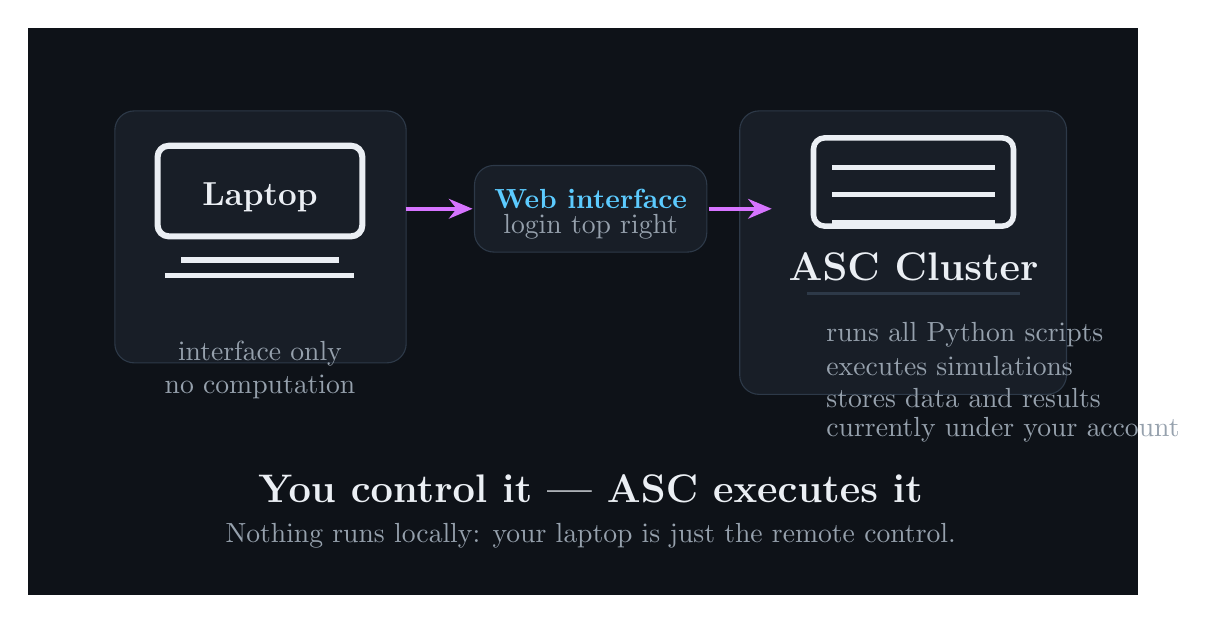
\begin{tikzpicture}[
  font=\sffamily\small,
  axis/.style={-{Stealth[length=3mm,width=2.5mm]}, line width=1.5pt, draw=MagentaAI},
  panel/.style={draw=calyrline, fill=calyrpanel, rounded corners=7pt},
  cardtitle/.style={text=calyrink, font=\bfseries\Large},
  body/.style={text=calyrmuted, font=\normalsize},
  accent/.style={text=calyraccent, font=\bfseries\normalsize}
]
\fill[calyrbg] (-0.3,-0.2) rectangle (13.8,7.0);

\node[panel, minimum width=3.7cm, minimum height=3.2cm, anchor=north west] (laptop) at (0.8,5.95) {};
\node[panel, minimum width=4.15cm, minimum height=3.6cm, anchor=north east] (cluster) at (12.9,5.95) {};

\draw[calyrink, line width=2.2pt, rounded corners=4pt] (1.35,4.35) rectangle (3.95,5.50);
\draw[calyrink, line width=2pt] (1.65,4.05) -- (3.65,4.05);
\draw[calyrink, line width=2pt] (1.45,3.85) -- (3.85,3.85);
\node[text=calyrink, font=\bfseries\large] at (2.65,4.85) {Laptop};
\node[body, align=center] at (2.65,2.65) {interface only\\no computation};

\draw[calyrink, line width=2pt, rounded corners=4pt] (9.68,4.48) rectangle (12.22,5.60);
\draw[calyrink, line width=1.8pt] (9.92,5.23) -- (11.98,5.23);
\draw[calyrink, line width=1.8pt] (9.92,4.88) -- (11.98,4.88);
\draw[calyrink, line width=1.8pt] (9.92,4.53) -- (11.98,4.53);
\node[cardtitle] at (10.95,3.96) {ASC Cluster};
\draw[calyrline, line width=1.2pt] (9.60,3.62) -- (12.30,3.62);
\node[body, align=left, anchor=west] at (9.72,3.10) {runs all Python scripts};
\node[body, align=left, anchor=west] at (9.72,2.70) {executes simulations};
\node[body, align=left, anchor=west] at (9.72,2.30) {stores data and results};
\node[body, align=left, anchor=west] at (9.72,1.90) {currently under your account};

\node[panel, minimum width=2.95cm, minimum height=1.1cm] (web) at (6.85,4.70) {};
\node[accent] at (6.85,4.83) {Web interface};
\node[body] at (6.85,4.48) {login top right};

\draw[axis] (4.5,4.70) -- (5.35,4.70);
\draw[axis] (8.35,4.70) -- (9.15,4.70);

\node[text=calyrink, font=\bfseries\Large, align=center] at (6.85,1.15) {You control it --- ASC executes it};
\node[body, align=center] at (6.85,0.55) {Nothing runs locally: your laptop is just the remote control.};
\end{tikzpicture}
\end{document}